\documentclass[12pt]{article}
%
\usepackage{amsfonts,amsmath,amssymb,enumerate,fancyhdr,fullpage,graphicx,hyperref,float,lastpage,multicol,multirow,pgfplots,setspace,subfigure,supertabular,tablefootnote,tikz, titlesec,vwcol,wasysym,xcolor}

\usepackage[bottom]{footmisc}
\usepackage[utf8]{inputenc}
\usepackage[backend=biber]{biblatex}

\newcounter{lemma}
\newcommand{\lemma}[0]{\textbf{Lemma \refstepcounter{lemma}\thelemma\label{lem:\thelemma}}}
\newcounter{corollary}
\newcommand{\corollary}[0]{\textbf{Corollary \refstepcounter{corollary}\thecorollary\label{cor:\thecorollary}}}
\newcounter{theorem}
\newcommand{\theorem}[0]{\textbf{Theorem \refstepcounter{theorem}\thetheorem\label{thm:\thetheorem}}}
\newcounter{defn}
\newcommand{\defn}[0]{\textbf{Definition \refstepcounter{defn}\thedefn\label{def:\thedefn}}}

\pgfplotsset{compat=newest}
\usetikzlibrary{shapes.geometric,arrows,fit,matrix,positioning}
\tikzset
{
    treenode/.style = {circle, draw=black, align=center, minimum size=1cm},
    subtree/.style  = {isosceles triangle, draw=black, align=center, minimum height=0.5cm, minimum width=1cm, shape border rotate=90, anchor=north}
}


\bibliography{quadtrees}
%
\hypersetup{colorlinks,citecolor=black,filecolor=black,linkcolor=black,urlcolor=black}
\titleformat{\section}
	{\normalfont\large\bfseries}
	{\thesection. }
	{0pt}{}
\titleformat{\subsection}
	{\normalfont\large\bfseries}
	{\thesubsection. }
	{0pt}{}
\titleformat{\subsubsection}
	{\normalfont\bfseries}
	{\thesubsubsection. }
	{0pt}{}
\titlespacing{\section}{0pt}{1em}{0em}
\setlength{\parskip}{1em}
\setlength{\parindent}{0cm}
\setlength{\columnsep}{1cm}
%
%begin document
\begin{document}
    \title{Analyzing Randomized and Deterministic Skip Quadtrees}
    \author{Botong Ma and William Qian\\\{btma, wqian94\}@mit.edu}
    \date{} % no date
    
    \maketitle
    
    \begin{abstract}
        \noindent Quadtrees and related spacial data structures have applications in modeling, machine learning, collision detection, and more. In this paper, we briefly discuss the skip quadtree data structure, then explore the two different variants described by Eppstein, Goodrich, and Sun \cite{sqt} through implementing both variants and comparing the results.
        
    \end{abstract}
    
    \section{Introduction} 
        \indent A quadtree is a tree where all the nodes can be visualized as a square divided into exactly four quadrants, representing the four children that each node has. When a collision occurs in one of the quadrants, it will then recursively split into four more nodes. Quadtrees are typically used to represent information in 2D, and are also often used for point and range queries. 
        
        Point query is a problem where given a set of $n$ points $S = {p_1, p_2, \hdots, p_n}$, we would like to quickly return the closest point $p_i$ in $S$ to a given point $q$ that may or may not be in $S$. In game design, this is often used for collision detection between objects. Range queries are directed at finding all points in a set $P$ that belong to a specific region. In both cases, quadtrees are useful for solving these problems. 
        
        Additionally, in graphics, meshes are used to define shapes of objects in modeling. Generally, they are composed of triangles or other simple shapes. However, sometimes, uniform meshes are not computationally sound for some objects, such as a model of a system of partial differential equations. In these cases, we will need a non-uniform mesh, which can be generated using a quadtree.
        
        Unfortunately, a na\"ive implementation of a quadtree can result in poor runtime and space bounds. In this paper, we begin at the na\"ive, simple quadtree and conclude by developing and testing tighter bounds for both runtime and space based on empirical data for skip quadtrees \cite{sqt}.

    \section{Background}
    \subsection{Terms}
        Before we begin, the reader should be familiar with two data structures, quadtrees \cite{qt} and skip lists \cite{sl}, as well as some associated terms.
        
        A \textit{simple quadtree} follows from the traditional definition of a quadtree $Q$ defined by its center point $q_0 = (x_0, y_0)$ and the side length $\ell_0$ of the region it bounds, where all quadrants have lengths exactly half of their parents (except the root). As a result, the upper bound on the tree's height has a dependency on the smallest pair-wise distances between two points in the tree, and the lower bound on the tree's height depends linearly on the number of points in the tree. The set of points contained by a quadtree is given by $p(Q)$ and the number of points in the quadtree is $n(Q) = |p(Q)|$.
        
        A \textit{skip list} is a 1D data structure that builds from a list $L_0$ of values, and keeps several ``levels" of the list as the lists $L_0, L_1, \cdots$, where $L_{i+1} \subseteq L_i$ for $i = 0, 1, \cdots$. The runtimes for inserting into, deleting from, and querying a skip list is, in expectation, $O(\lg n)$, if $L_0$ has $n$ elements. The space required to store a skip list is $O(n)$ if a point $p_j \in L_i$ exists also in $L_{i+1}$ with a fixed probability.
        
        A \textit{node} is an element in the tree. Each node can have a key (or value), children, and a parent. Each node is always the parent for its children, and a child for its parent.
        
        A \textit{leaf node} is a node with no children in the tree.
        
        An \textit{internal node} is a node with children in the tree.
        
        The \textit{root node} of a tree is the node with no parent. Since an empty tree has no root, the root node is always an internal node.
        
    \subsection{Simple Quadtrees}
%        Consider the 1D region $R$ of length $\ell_0$ centered at point $q_0$. We know this as the range from $q_0-\frac{1}{2}\ell_0$ to $q_0+\frac{1}{2}\ell_0$ on the real number line. 
%        
%        
%        \begin{figure}[ht!]
%            \centering
%            \begin{tikzpicture}[scale=2]
%                \draw[very thick] (-1,0) -- (1,0);
%                \path [draw=black, fill=black] (1,0) circle (2pt);
%                \path [draw=black, fill=black] (-1,0) circle (2pt);
%                \path [draw=black, fill=white, thick] (-0.2, 0) circle (2pt) ;
%                \path [draw=black, fill=white, thick] (-0.4, 0) circle (2pt);
%                \path [draw=black, fill=white, thick] (0.5, 0) circle (2pt);
%                \path [draw=black, fill=white, thick] (0.1, 0) circle (2pt);
%                \path [draw=black, fill=white, thick] (0.8, 0) circle (2pt);
%                \path [draw=black, fill=white, thick] (-0.7, 0) circle (2pt);
%                \draw[latex-latex] (-3.5,0) -- (3.5,0) ;
%                \foreach \x in  {-3,-2,-1,0,1,2,3}
%                \draw[shift={(\x,0)},color=black] (0pt,3pt) -- (0pt,-3pt);
%                \foreach \x in {-3,-2,-1,0,1,2,3}
%                \draw[shift={(\x,0)},color=black] (0pt,0pt) -- (0pt,-3pt) node[below] 
%                {$\x$};
%            \end{tikzpicture}
%            \label{fig:1}
%            \caption{An example region where $n=6$, $q_0 = 0$ and $\ell_0 = 2$.}
%        \end{figure}
%        
%        If we then have $n$ points $p_1,\cdots,p_n$ from within this range, we can construct a binary search tree to store these $n$ points. While many methods exist for constructing such a tree, one such method uses our knowledge that the points are contained in $R$.
%        \begin{figure}[ht!]
%            \centering
%                \begin{tikzpicture}[->,>=stealth', level/.style={sibling distance = 5cm/#1, level distance = 1.5cm}, scale=0.6,transform shape]
%                    \node [treenode] {$p_1$}
%                    child
%                    {
%                        node [treenode] {$p_2$} 
%                            child
%                            {
%                                node[treenode] {$p_3$}
%                            }
%                            child
%                            {
%                                node[treenode] {$p_4$}
%                            }
%                    }
%                    child
%                    {
%                        node[treenode] {$p_5$}
%                        child
%                        {
%                            node [treenode] {$p_6$}
%                        }
%                    };
%                
%                \end{tikzpicture}
%            \label{fig:2}
%            \caption{Binary tree for the example region in Figure \ref{fig:1}}
%        \end{figure}
%        
%        Let the entire tree contain all the points with the root's key being $q_0$, then divide $R$ into two equal subspaces, $R_1$ and $R_2$. Define the left subtree to contain all points in $R_1$ and the right subtree to contain all points in $R_2$, and each corresponding internal node's key being the center of the region that its subtree represents. We can then recursively define our tree this way, letting only leaves.
%        
%        As stated before, a quadtree $Q$ is a geometric data structure where each node can be visualized as a square, and has exactly four children.  
        \subsubsection{QUERY}
            The worst-case scenario for a simple quadtree centered at $q_0 = (x_0, y_0)$ with side length $\ell_0$ can be achieved with just two points: $p_1 = (x_0 + \varepsilon, 0)$ and $p_2 = (0, y_0 + \varepsilon)$ for $\varepsilon > 0$. Inserting just these two points in the quadtree will result in $\approx \lg \frac{\ell_0}{2\varepsilon}$ subdivisions before $p_1$ and $p_2$ end up in separate quadrants, which means that both points are at depth $O(\lg \frac{\ell_0}{2\varepsilon}) = O(-\lg \varepsilon)$ for a fixed $\ell_0$. Then, as $\varepsilon \to 0$, it is easy to see that we asymptotically approach infinite depth, and thus, asymtotically-infinite search time in the worst case.
        \subsubsection{INSERT}
            Since inserting implicitly involves traversal, insertion inherits the same worst-case asymptotically-infinite runtime for points that are clustered very closely together.
        \subsubsection{DELETE}
            Similarly, deletion also incurs, in the worst-case scenario, asymptotically-infinite runtime.
        
    \subsection{Compressed Quadtrees}
        As we just saw, the worst-case runtimes for a simple quadtree have a dependency on the pairwise distances between the points, resulting in the possibility of an asymptotically-infinite runtime for all three functions. To eliminate this awful dependency, we make the following observation: the asymptotically-infinite runtimes result from the asymptotically-infinite depth, which in turn results from having so many non-splitting internal nodes. These nodes have only one child, and as it turns out, we need not keep track of all these internal nodes.
        
        A \textit{compressed quadtree} \cite{cqt} is like a simple quadtree, except with one additional rule: excluding the root, all internal nodes must contain at least two children (the root is allowed to have only 1 child). Conceptually, this means that if a quadrant has only one child, it will be replaced by that child, such that the parent points directly to the child, rather than to this quadrant. Recursively applying this idea, we can see that a compressed quadtree is still correct, while requiring less space in memory.
        
        \lemma: Inserting a point into a compressed quadtree $Q$ adds at most two nodes to $Q$.
        
        \textbf{Proof:} If $Q$ is empty, then it has no nodes, so when we add a point $p$ into $Q$, we must add one node for the root node and one node for the point.
        
        If $Q$ is not empty, then when we insert a point into $Q$, we must create one node to represent the point, and if a collision occurs, we must resolve that collision. Since every non-root internal node must have at least two children, we only create one internal node to resolve each collision.
        
        This means that, for each point we insert, we will also create at most one internal node. Thus, inserting a point in the tree results in an addition of at most two nodes to the tree. \hfill $\blacksquare$
        
        \theorem: A quadtree of $n$ points has at most $2n$ nodes.
        
        \textbf{Proof:} By Lemma \ref{lem:1}, we know that each insertion increases the node count by at most 2, so after inserting $n$ nodes into an initially-empty tree, the tree has at most $2n$ nodes. \hfill $\blacksquare$
        
        Therefore, a compressed quadtree of $n$ points requires only $O(n)$ space, which is an improvement on the simple quadtree, now that we have eliminated the dependency on the smallest pairwise distances between the points.
        
        \begin{figure}[ht!]
            \centering
          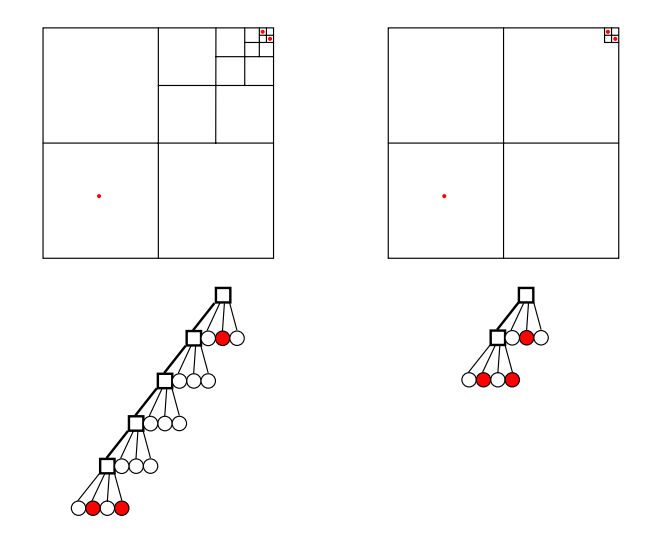
\includegraphics[scale=0.75]{CompressedQuadtree.png}
          \caption{A simple quadtree (left) and the corresponding compressed quadtree (right), taken from Figure 1 in \cite{sqt}.}
          \label{fig:3}
        \end{figure}
        
        \subsubsection{QUERY}
            From Theorem \ref{thm:1}, we know that, after inserting $n$ points, the tree can have at most $2n$ nodes. Since exactly $n$ of these nodes must be leaf nodes, this mean that a tree can have at most $n$ internal nodes, so the tree has height at most $n$. This occurs when all $n$ points are constructed such that $p_j = (x_0 + \ell_0 (1 - 2^{-j}), y_0 + \ell_0 (1 - 2^{-j}))$ for $j = 1, \cdots, n$. With such a construction for the $n$ points, the tree will have height $n$, so the worst-case runtime for querying a compressed quadtree is $O(n)$.
            
        \subsubsection{INSERT}
            Inserting a point into a compressed quadtree requires a traversal and then actually creating and inserting the nodes. By Lemma \ref{lem:1}, we know that an insertion requires the creation of a constant number of nodes. We can then see that we also only need to change a constant number of pointers, so the actual creation and insertion of the nodes takes constant time. Since we have just shown that a traversal takes $O(n)$ time, this means that the runtime for inserting a point in a quadtree is $O(n)$.
            
        \subsubsection{DELETE}
            Deleting a point requires a traversal followed by disconnecting the node representing the point from the rest of the tree. Such a disconnection might also trigger the deletion of the parent node as well, so we might have to delete two nodes from the tree; fortunately, we will never have to delete the grandparent node because by virtue of having a parent, the node must also have a sibling, so that sibling will replace the parent if the parent is also deleted, which does not change the number of children that the grandparent has. Thus, the actual deletion of up to two nodes from the tree is $O(1)$, so the overall runtime for a deletion is dominated by the traversal, which is $O(n)$.
        
    \section{Skip Quadtrees}
        A skip quadtree takes the idea of skip lists and applies it to compressed quadtrees. Instead of having layers of lists, we instead have layers of quadtrees, denoted by $Q_i$, where $i \geq 0$ indicates the level of the quadtree \cite{sqt}. $Q_0$ is the original compressed quadtree, which contains all the points in the data structure.
        
        \defn: In a skip quadtree, if $b > a$, then $p(Q_b) \subseteq p(Q_a)$.
        
        \theorem: If node $v \in Q_{i+1}$, then we know that $v \in Q_i$.
        
        \textbf{Proof:} We will consider $v$ in two scenarios: $v$ is a leaf node and $v$ is an internal node.
        
        Consider when $v$ is a leaf node. Then by Definition \ref{def:1}, we know that $v \in Q_{i+1} \implies v \in Q_i$, so this case is trivial.
        
        Consider when $v$ is an internal node. This means that $v$ has at least two children, implying that $\exists p_1, p_2$ such that $p_1$ and $p_2$ are points that belong to different subquadrants of $v$, and correspond to leaf nodes. This means that $p_1$ and $p_2$ certainly must exist in $Q_i$, so it must be necessary to have $v$ in $Q_i$ to resolve the collision that would otherwise occur between $p_1$ and $p_2$ in $Q_i$.
        
        Thus, we can conclude that, if $v \in Q_{i+1}$, then $v \in Q_i$. \hfill $\blacksquare$
        
    \subsection{Promotion and Demotion}
        
        If $p_j \in Q_i$ but $p_j \not\in Q_{i+1}$, then the process of adding $p_j$ to $Q_{i+1}$ is called \textit{promotion}. Similarly, if $p_j \in Q_i$ and $Q_{i+1}$, then the process of removing $p_j$ from just $Q_{i+1}$ is called \textit{demotion}. This leads us to the following decision problem.
        
        \defn\ (The Promotion Problem): Given a point $p_j$ such that $p_j \in Q_i$ and $p_j \not\in Q_{i+1}$, should $p_j$ be promoted to $Q_{i+1}$?
        
        Below, we examine the two variants of skip quadtrees that \cite{sqt} describes: randomized and deterministic. These terms refer to the algorithm used to decide the Promotion Problem. Interestingly, the applications of the Promotion Problem also differ between these two variants.
    
    \subsection{Randomized Skip Quadtrees}
        The randomized skip quadtree decides the Promotion Problem in a probabilistic manner. Define $P$ to be the probability that we answer the Promotion Problem with YES. Then, each time we insert a point $p_j$, we ask for decisions to the Promotion Problem until we get a NO. Letting $k$ be the number of times we got YES before we got NO, then $p_j$ should be promoted $k$ times from $Q_0$, such that $p_j \in Q_0, \cdots, Q_k$.
        
        This means that, for a skip quadtree of $n$ points,
        $$\mathbb{E}[n(Q_i)] = n \cdot P^{-i} \implies \mathbb{E}[|Q_i|] \leq 2n \cdot P^{-i},$$
        so the expected number of nodes overall in the skip quadtree is
        $$\mathbb{E}[|Q|] = \sum_{i = 0}^\infty \mathbb{E}[|Q_i|] \leq \sum_{i = 0}^\infty (2n \cdot P^{-i}) = \frac{2n}{1 - P} = O(n).$$
        So, we can expect query, insertion, and deletion operations to run in $O(\lg n)$ time while still using only linear space \cite{sqt}.
        
        \begin{figure}[ht!]
            \centering
          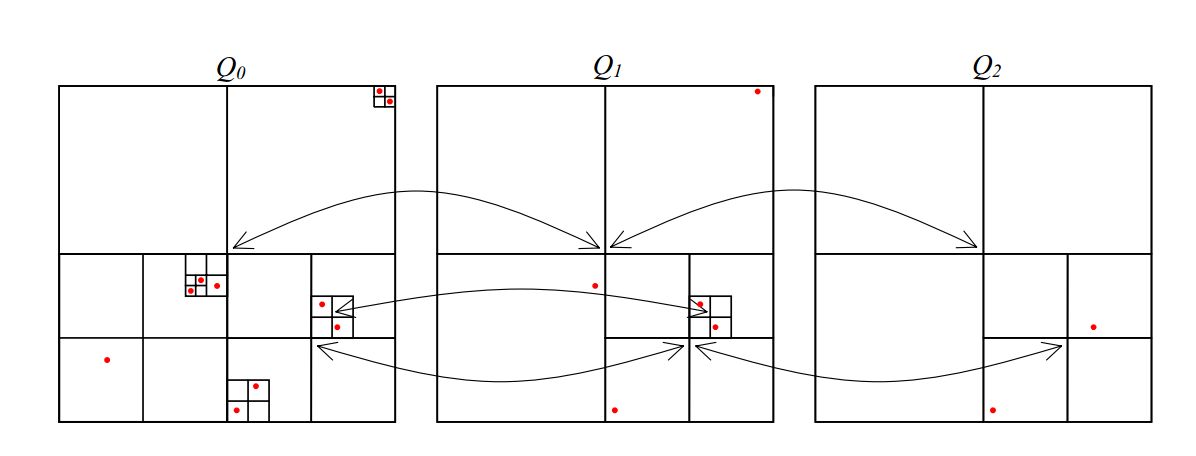
\includegraphics[scale=0.75]{RandomizedCompressedQuadtree1.png}
          \caption{Randomized skip quadtree layers, Figure 2 in \cite{sqt}.}
          \label{fig:4}
        \end{figure}
         
    \subsubsection{Analysis}
        Unfortunately, randomized skip quadtrees do not entirely solve the problem. While \textit{on expectation} the quadtree can query, insert, and delete in $O(\lg n)$ time, there still exists the possibility of randomization working against us. For example, suppose we used the data set described in section 2.3.1; then, with probability $(1 - P)^{-n}$, no points will be promoted from $Q_0$ to $Q_1$, so we are left with essentially the same situation as in 2.3.1, 2.3.2, and 2.3.3: linear runtime.
        
        Another problem with randomized skip quadtrees is that the number of levels is unbounded, and as a result, for any point being inserted, it is possible to end up with far more levels than necessary.
        
    \subsection{Deterministic Skip Quadtrees}
        The deterministic skip quadtree resolves the problem posed by the poorly-chosen data set above. To do this, the deterministic skip quadtree adds an additional invariant to the mix: the leaf nodes must form a valid 1-2-3 skip list \cite{dsl}. Note that forming such a skip list requires a total order of the points, and one such ordering is by comparing points dimension-by-dimension.
        
        By applying the insertion and deletion principles of 1-2-3 skip lists from \cite{dsl} to skip quadtrees, insertion and deletion operations on deterministic skip quadtrees achieve a deterministic runtime of $O(\lg n)$ \cite{sqt}.
    
    \section{Implementation}
        In order to compare randomized and deterministic skip quadtrees, we decided to implement both data structures and compare their benchmark results. For the purposes of this paper, we implemented and compared only the query and insertion operations. Since the deletion operations are the most difficult to implement and we would expect to see roughly the same results as with insertion operations, we chose to leave deletion operations out of our implementation and comparisons.
        
        We implemented both variants in C, for performance reasons, and used a common interface to ensure that the data structures and functions are comparable. In both cases, the query and insertion operations are implemented recursively.
        
        Additionally, for the randomized implementation, we set $P = \frac{1}{2}$, so each node has a $\frac{1}{2}$ probability of being promoted.
    
    \section{Benchmark}
    \subsection{Hardware Specifications}
        We ran our benchmarks on a machine with 16 Intel\textsuperscript\textregistered\ Core\textsuperscript\texttrademark\ i7-5960X cores, each running at 3 GHz, hosted by MIT's Computer Science and Artificial Intelligence Laboratory. Since our benchmarks were single-threaded, we only used one of the cores.
    
    \subsection{Methods}
        The benchmark reports throughput, measured by the number of completed operations, given a time interval, the number of dimensions, an initial population count, and the probability of running an insertion operation (as opposed to a query operation). The initial population count parameter determines the initial size of the tree before benchmarking begins -- the larger this value, the lower the probability of collisions. The insertion operation probability determines approximately how many of the total operations will be insertion operations -- the remaining operations are all queries.
        
        Although the points are generated randomly, the random number generator is seeded deterministically, such that at least the initial population is the same for runs with the same initial population count. The random number generator we used is an implementation of the Marsaglia polar method, which we believe produces a sufficiently-uniform distribution for our purposes.
        
        Hardware-wise, since we ran these benchmarks on the same dedicated machine, we have high confidence in our results.
        
    \subsection{Results}
        We chose to fix the time intervals at 1 second, and the number of dimensions at 2. We then varied the initial population count parameter by choosing an initial population of 1, 1000, and 1000000 nodes, while also varying the insertion operation probability by choosing 0\%, 1\%, and 10\%. We then ran each trial five times, and took the average of the results to produce Table \ref{tbl:1}.
        
        \begin{table} [ht!]
        \centering
            \begin{tabular}{|r|r|r|r|r|}
            \hline
            \textbf{Nodes}& \textbf{\% Insertions}& \textbf{Randomized}& \textbf{Deterministic}& \textbf{Ratio: R/D}\\ \hline
            1       & 0\%           &    20746759 &    15851391    & 1.31       \\ \hline
            1       & 1\%           &    5794683  &    14607628    & 0.40       \\ \hline
            1       & 10\%          &    2416052  &    7743879     & 0.31       \\ \hline
            1000    & 0\%           &    11733530 &    15610295    & 0.75       \\ \hline
            1000    & 1\%           &    3150763  &    4866744     & 0.65       \\ \hline
            1000    & 10\%          &    1661835  &    3476177     & 0.48       \\ \hline
            1000000 & 0\%           &    6533244  &    15614092    & 0.42       \\ \hline
            1000000 & 1\%           &    2386309  &    3133555     & 0.76       \\ \hline
            1000000 & 10\%          &    1489428  &    2767394     & 0.54       \\ \hline
            \end{tabular}
            \label{tbl:1}
            \caption{Results of the benchmark, averaged over five trials. Note that the deterministic implementation consistently outperforms the randomized implementation, except for the single-node-query-only test case.}
        \end{table}
        
    \section{Discussion}
        From Table \ref{tbl:1}, we can see that, of the 9 test cases, the deterministic implementation outperforms the randomized implementation in 8 test cases. The only test case where the randomized implementation performs better is the test case where the tree begins with only 1 point, and the benchmark tests only for query operations. This is a little surprising because the algorithms used in both implementations for querying are the same. One possible explanation for this behavior is that the deterministic implementation has no nodes at the top-most level of the tree, so when querying, we always have to drop down a level to reach a non-empty level; on the other hand, the randomized version does not have this layer, and thus when only 1 point is in the tree, that point can be found without needing to recurse down a level.
        
        For the other 8 test cases, the fact that the deterministic implementation outperforms the randomized implementation is surprising. We had initially hypothesized that the randomized implementation would perform better, due to having to preserve fewer invariants, which resulted in less logic in the code for the randomized implementation. The actual data, however, belies this hypothesis, and additionally shows that, in fact, the deterministic implementation severely outperforms the randomized one.
        
        As we can see in Figures \ref{fig:3}, \ref{fig:4}, and \ref{fig:5} in the Appendix, whenever insertions became involved, the deterministic implementation produced faster runtimes per operation compared to the randomized implementation, and held this lead as the number of initial nodes increased. This suggests that inserting a point may be significantly faster with the deterministic implementation than with the randomized one. This is perhaps due to how the answer to the Promotion Problem is decided. For the randomized implementation, the decision is to promote with $\frac{1}{2}$ probability, so on expectation, after $n$ insertions, we will have promoted $n$ times. On the other hand, for the deterministic implementation, promotions only occur when 3 nodes are already adjacent in a given level \cite{dsl}. This means that promotions happen once for every fourth node inserted in a row, so after $n$ insertions, we can expect about $\frac{n}{2}$ promotions. While the factor of 2 is small at face value, it results in significant performance differences because insertions, which mutate the data structure, are far more expensive than queries, which are read-only operations.
        
        Additionally, it is also worthwhile to note that, with the exception of the deterministic implementation for 0\% insertions, all the other graphs support the claim that both implementations sport $O(\lg n)$ runtimes for their query and insertion operations. Moreover, the slopes are incredibly modest, which suggests that the constant is manageable and the data structures are feasible.
        
        That said, it is also important to note the behavior of the deterministic implementation for 0\% insertions. Unlike all the other trends, this one remains constant, regardless of how many initial nodes there are. This seems suspicious, and warrants further investigation to determine the cause of this unusual behavior.
        
        Unfortunately, the efficiency of the deterministic implementation is undercut by is noticeably-more-difficult implementation, which requires not only the quadtree itself, but also an underlying 1-2-3 skip list.
    
    \section{Conclusion}
        Compared to the simple quadtree, both the randomized and deterministic implementations of the skip quadtree perform far better and can better handle worst-case scenarios for the simple quadtree. We also used the empirical data to validate the authors' claim that skip quadtrees have $O(\lg n)$ query and insertion operations \cite{sqt}.
        
        Between the randomized and deterministic implementations themselves, although we had originally believed that the randomized implementation would be more performant than the deterministic implementation due to the latter implementation's need to also build a 1-2-3 skip list, empirical results showed that, in fact, the deterministic implementation outperforms the randomized one in most cases.
        
    \section{Future Work}
        In this exploration into skip quadtrees, our implementations for both the randomized and deterministic have not been performance engineered. As a result, it is possible that well-tuned and better-engineered implementations may produce different results regarding the relative efficiencies of these data structures. Additionally, we did not compare the deletion operations for these quadtrees, so a future work may consider implementing the deletion operation and comment on the performance and implementation results. Finally, further comparison with other spacial data structures, such as k-d trees, will be necessary to fully determine the scope for which skip quadtrees are optimal.
    
    \pagebreak
    
    \section{Appendix}
        
    \begin{figure}[ht!]
        \centering
        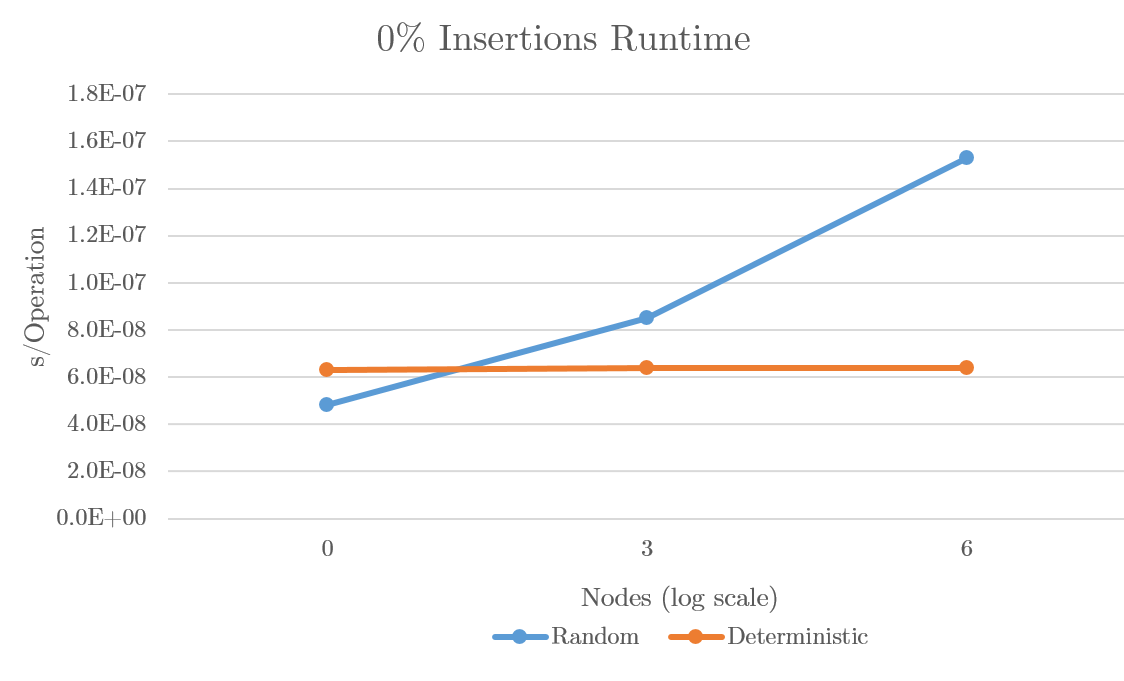
\includegraphics[scale=1.0]{0Insertion.png}
        \caption{Comparison of 0\% Insertion Runtimes}
        \label{fig:5}
    \end{figure}
         
    \begin{figure}[ht!]
        \centering
        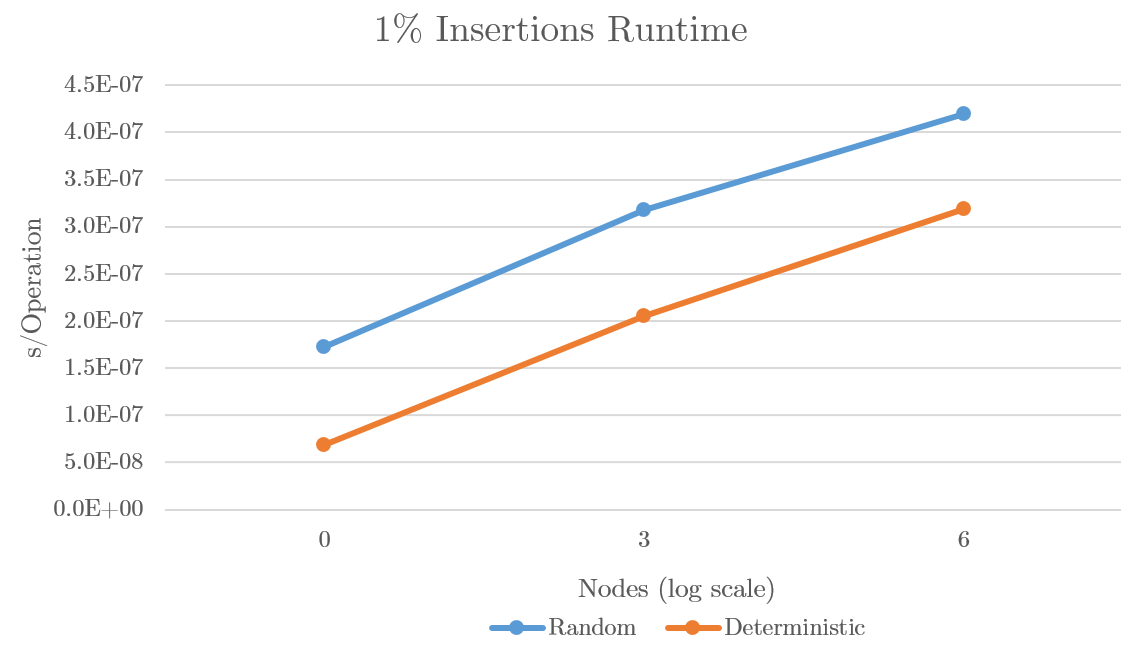
\includegraphics[scale=1.0]{1Insertion.png}
        \caption{Comparison of 1\% Insertion Runtimes}
        \label{fig:6}
    \end{figure}
         
    \begin{figure}[ht!]
        \centering
        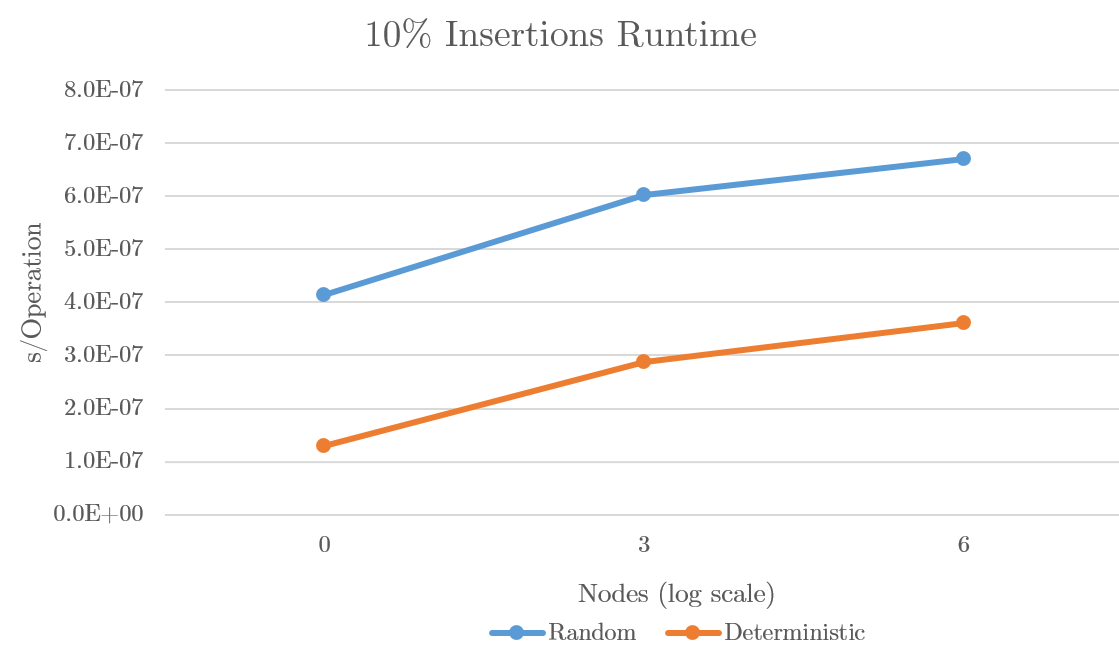
\includegraphics[scale=1.0]{10Insertion.png}
        \caption{Comparison of 10\% Insertion Runtimes}
        \label{fig:7}
    \end{figure}

    % bib stuff
    \printbibliography
\end{document}